%(BEGIN_QUESTION)
% Copyright 2011, Tony R. Kuphaldt, released under the Creative Commons Attribution License (v 1.0)
% This means you may do almost anything with this work of mine, so long as you give me proper credit

Studer denne {\it ventilsignaturen} fra en ventil som tydelig har problemer, og svar på spørsmålene under:

$$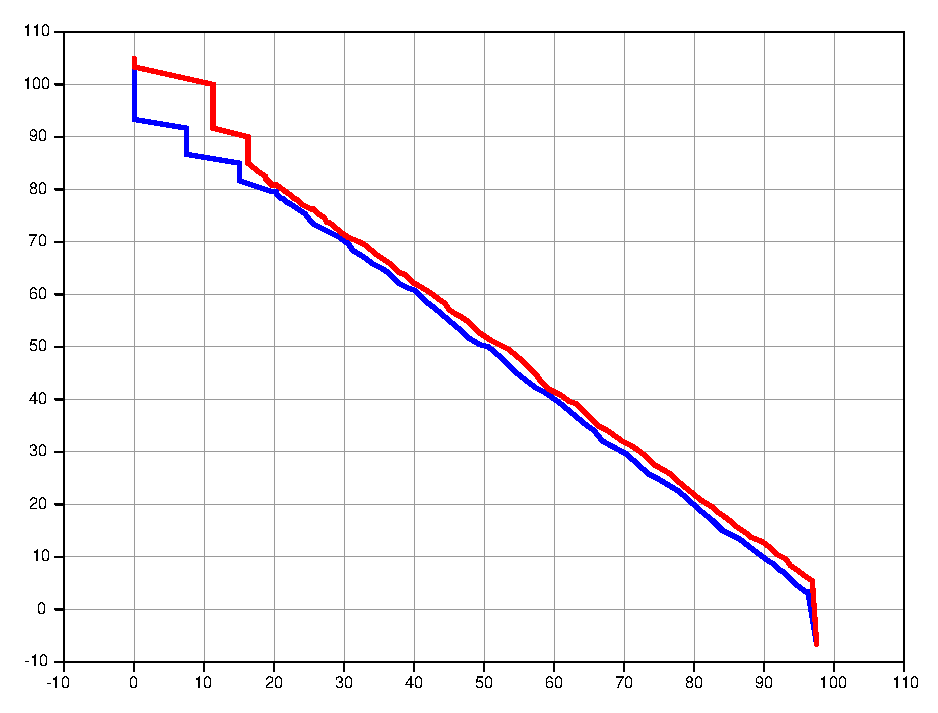
\includegraphics[width=15.5cm]{i00426x01.eps}$$

\begin{itemize}
\item{} Er dette en luft-åpne-ventil eller en luft-lukke-ventil?
\vskip 10pt
\item{} Hvilken akse i grafen (horisontal eller vertikal) representerer (prosent av) ventilspindelens posisjon?
\vskip 10pt
\item{} Hvilken akse i grafen (horisontal eller vertikal) representerer (prosent av) aktuatorens lufttrykk?
\vskip 10pt
\item{} Hvilken type problem har denne ventilen, og hvordan kan det utbedres?
\end{itemize}

\underbar{file i00426}
%(END_QUESTION)




%(BEGIN_ANSWER)

\noindent
{\bf Delvis svar:}

\begin{itemize}
\item{} Er dette en luft-åpne-ventil eller en luft-lukke-ventil? {\it Det er en luft-lukke-ventil. Vi ser det av negativ helning i kurvene: høyere lufttrykk kreves for å bevege ventilspindelen lenger mot lukket stilling.}
\vskip 10pt
\item{} Hvilken akse i grafen (horisontal eller vertikal) representerer (prosent av) ventilspindelens posisjon? {\it Den horisontale aksen. Dette ser vi av de bratte «ned»- og «opp»-svingene i hver ende av kurvene: her får vi trykkspiker i aktuatoren med liten eller ingen spindelbevegelse fordi spindelen har nådd mekanisk endestopp.}
\end{itemize}

%(END_ANSWER)





%(BEGIN_NOTES)

\begin{itemize}
\item{} Er dette en luft-åpne-ventil eller en luft-lukke-ventil? {\it Det er en luft-lukke-ventil. Vi ser det av negativ helning i kurvene: høyere lufttrykk kreves for å bevege ventilspindelen lenger mot lukket stilling.}
\vskip 10pt
\item{} Hvilken akse i grafen (horisontal eller vertikal) representerer (prosent av) ventilspindelens posisjon? {\it Den horisontale aksen. Dette ser vi av de bratte «ned»- og «opp»-svingene i hver ende av kurvene: her får vi trykkspiker i aktuatoren med liten eller ingen spindelbevegelse fordi spindelen har nådd mekanisk endestopp.}
\vskip 10pt
\item{} Hvilken akse i grafen (horisontal eller vertikal) representerer (prosent av) aktuatorens lufttrykk? {\it Den vertikale aksen, av samme grunn som over.}
\vskip 10pt
\item{} Hvilken type problem har denne ventilen, og hvordan kan det utbedres? {\it Det er svært høy friksjon i ventilmekanismen mot lukket (setende) posisjon. Enten er trimmen mekanisk skadet, eller så er ventilen feilmontert.}
\end{itemize}

%INDEX% Final Control Elements, valve: diagnostic signature for pneumatic actuator

%(END_NOTES)
